\documentclass{article}
\usepackage[utf8]{inputenc}
\usepackage[english]{babel}
\usepackage[T1]{fontenc}
\usepackage[a4paper]{geometry}
\usepackage{natbib}
\usepackage{graphicx}
\usepackage{amsmath}


\begin{document}
\renewcommand{\contentsname}{Indice}

\newcommand{\createEquation}[1]{
	\vspace{0.5cm} 
	\begin{equation}
		{#1}
	\end{equation}
	\vspace{0.5cm}
}


\title{Internal forces in liquids}
\author{Milos Bondi and Leonardo Saurwein}
\date{2022}

\newcommand\blankpage{
\null
\thispagestyle{empty}
\addtocounter{page}{-1}
\newpage
}

\newcommand{\Hrule}{\rule{\linewidth}{0.5mm}}

\begin{titlepage} %Pagina titolo
		\center
		\textsc{\LARGE ETHZ} \\[0.7cm] % nome scuola
		{\large 10.03.2022} \\[1cm]
		\begin{figure}
		    \centering
		    
\includegraphics[scale=0.2]{logo_ethz.png}
		\end{figure}
		
		\textsc{\Large D-PHYS} \\ [0.5cm]%corso/lavoro
		
		\Hrule \\ [0.4cm]
		{\huge \bfseries Internal forces in liquids} \\[0.4cm] %titolo LAM
		\Hrule \\[0.4cm]
		
		\begin{figure}[h!]
		    \centering
		    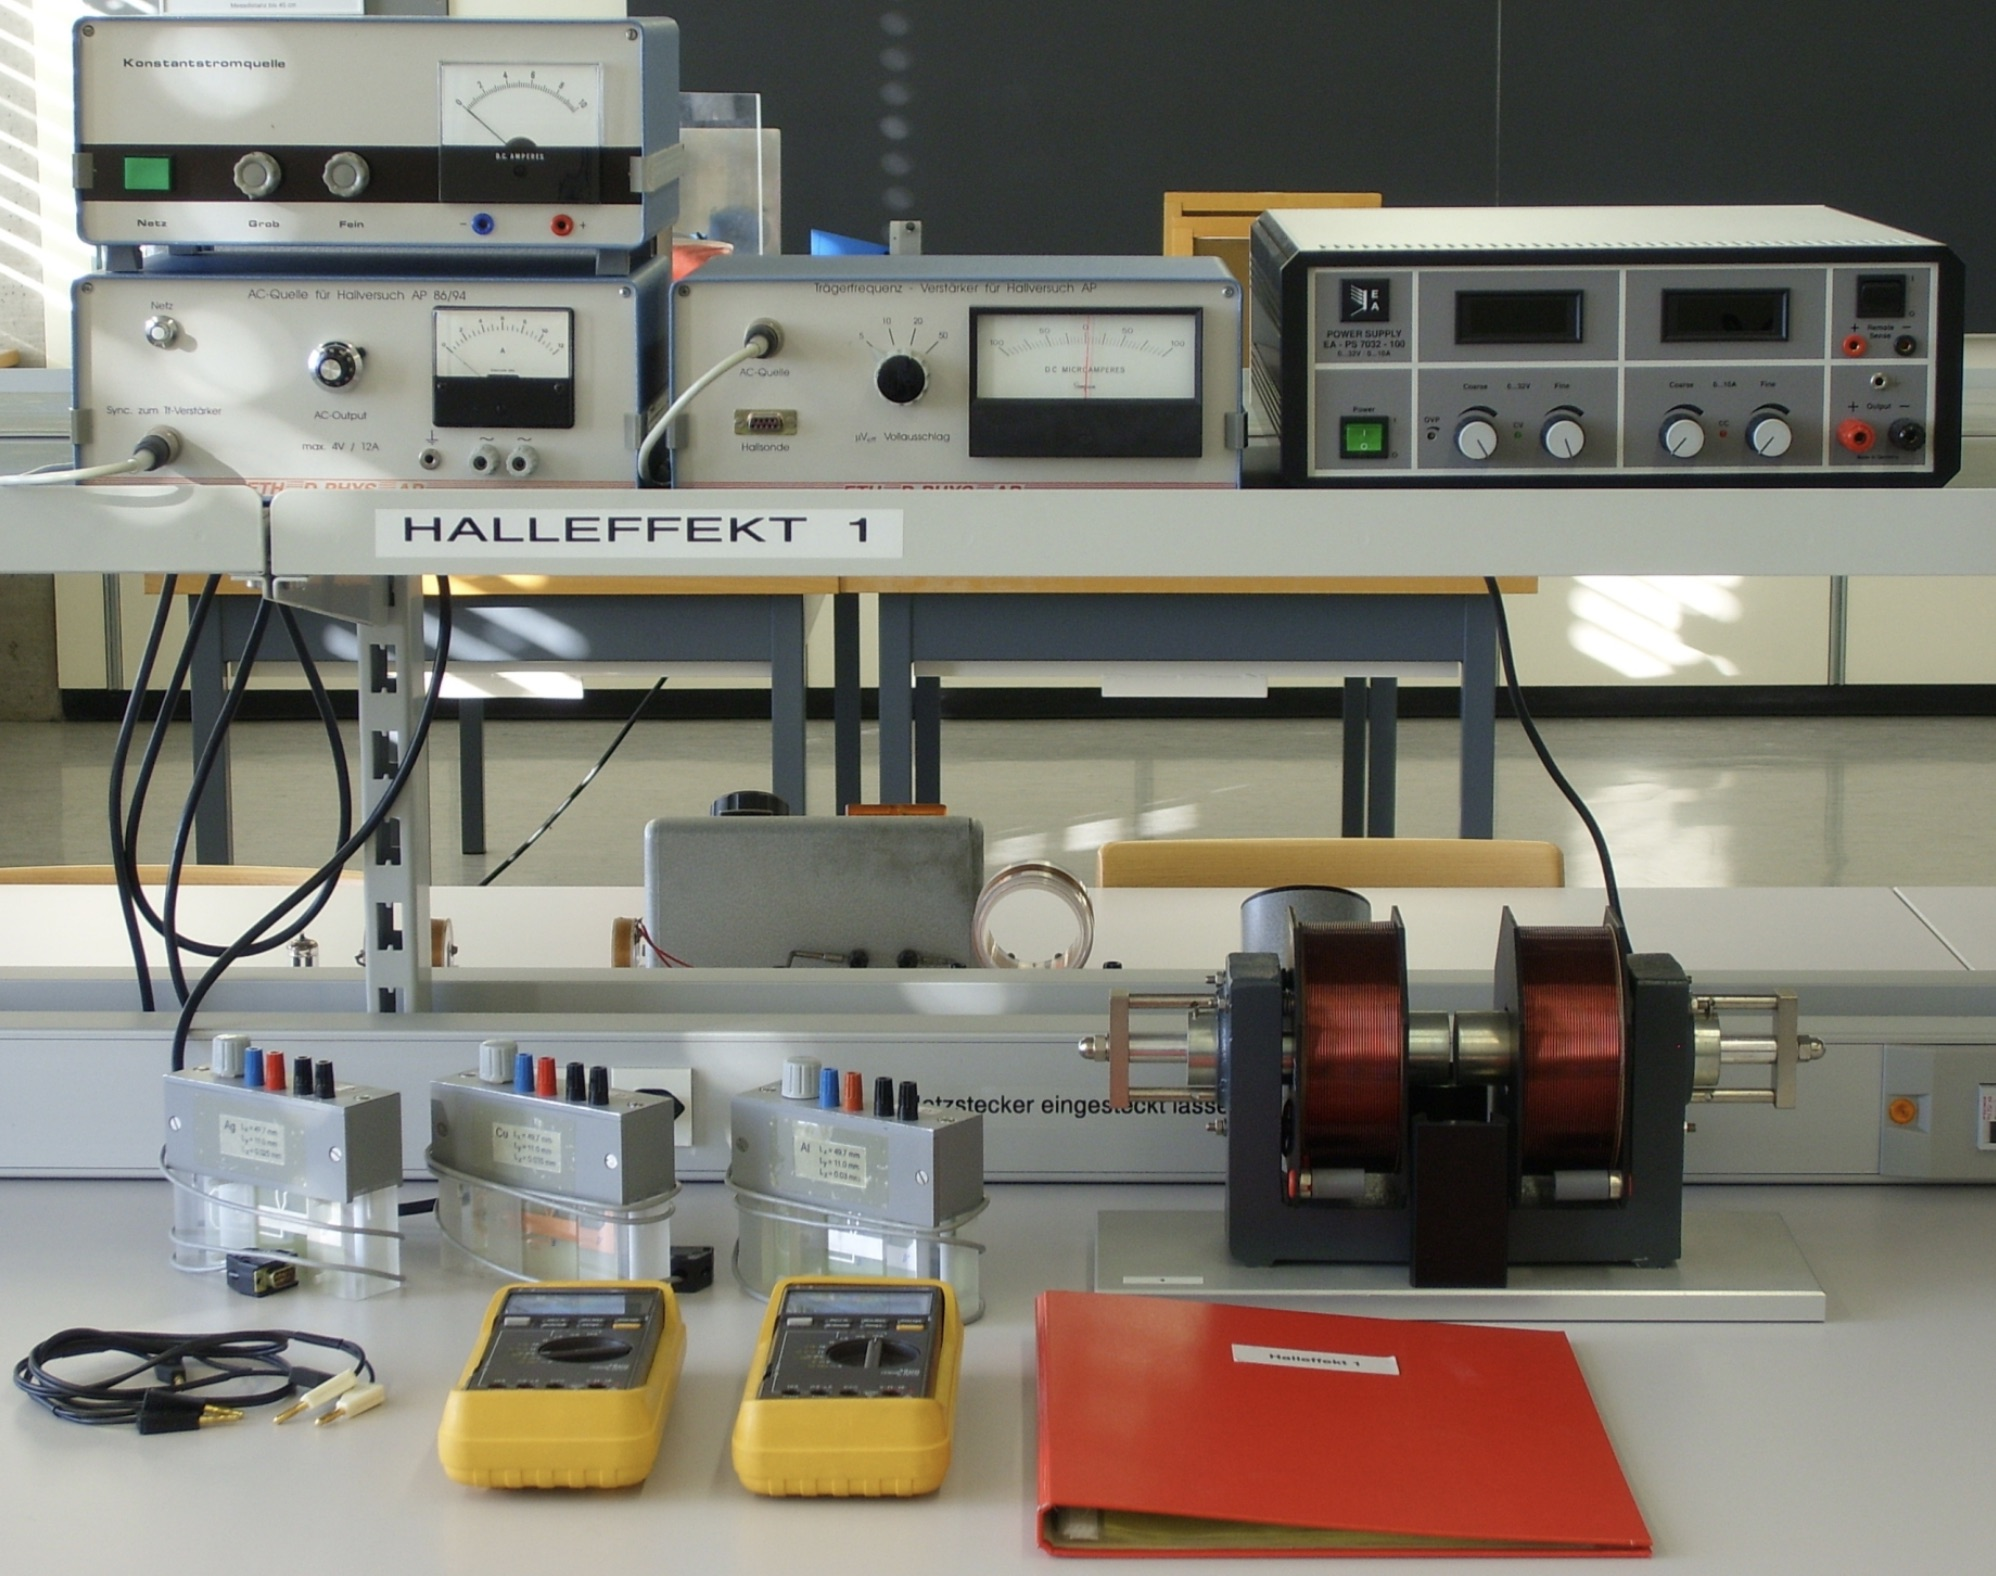
\includegraphics[scale=0.10]{39_Preview.jpg}
		\end{figure}
		
		\begin{minipage}{0.4\textwidth}
			\begin{flushleft} \large
				\emph{Authors:}\\
				Corti \textsc{Christian} \\ ccorti@student.ethz.ch \\ 20-928-479 \\
				\vspace{1mm}
				Leonardo \textsc{Saurwein} \\lsaurwein@student.ethz.ch \\20-927-745
			\end{flushleft}
		\end{minipage}
		~
		\begin{minipage}{0.5\textwidth}
			\begin{flushright} \large
				\emph{Supervisor:} \\
				Dante \textsc{Zanuz} \\ dzanuz@ethz.ch %SUPERVISORI
			\end{flushright}
		\end{minipage}\\[2cm]
		\vfill
\end{titlepage}

\newpage

\tableofcontents{}

\newpage

\section{Introduction}
The Hall effect is an electromagnetic effect discovered in 1879 by scientist E. Hall. Hall. It refers to the voltage measurable across a conductor (or semiconductor), when an electric current flowing through it is influenced by a magnetic field.
In summary: the Hall effect, relates to the formation of a potential difference between the opposite faces of an electrical conductor; this difference is attributable to a magnetic field that is perpendicular to the flow of electric current. \par
The fundamental physical principle behind the Hall effect is the Lorentz force. When an electron moves along a direction, v, perpendicular to the applied magnetic field, B, it experiences a force, F, the Lorentz force.
In response to this force, the electrons move in a curved path along the conductor and a net charge, and thus a voltage, develops across the plate.\par
Our task in this lab is

\begin{enumerate} % Da cambiare con i punti da fare
	\item Measure the conductivity of thin films of copper, silver and aluminum without external magnetic field
	\item Determine with the Hoeppler viscometer the viscosity for oil of the density $0.90\times10^{3} kgm^{3}$ as function of the temperature between 25°C and approx. 50°C and give a graphic representation of the function: $\eta = f(T)$
	\item Measure the tensile force $F_{w,max}$ at which a liquid lamella breaks off an aluminum ring, and then calculate the surface tension of the liquid. The liquids used are water and water with detergent.
	\item The surface tension of water should also be determined using the capillary rise method. 
	\item Compare the two methods to determine $\sigma $, argue which method is more accurate, why and where the biggest error or uncertainty comes from.
	\item Confirm the resistance law for turbulent flow on a cylindrical test body and calculate its resistance number $C_{W}$ . Present $W$ graphically as a function of $v^{2}: W = f(v^{2})$
\end{enumerate}

\newpage

\section{Task 1: Conductivity of Metal Foils}
Using a constant current of 5A and the formula shown below, we have calculated the conductivity of different metal foils. 
\createEquation{
	\sigma  = \frac{I_{x}L_{x}}{V_{x}L_{y}L_{z}}
	}

\noindent The parameters $L_{x}, L_{y}$ and $L_{z}$ are given from the object in the table below are marked down the value as well the final value of the conductivity of the different metal foils

\begin{table}[h]
	\caption{Experiment results}
	\vspace{0.1cm}
	\centering
	\begin{tabular}{c c c c c c}
		\hline\hline
		Material & $L_{x} [mm]$ & $L_{y}[mm]$ & $L_{z}[mm]$ & $V_{x}[mV]$ & $\sigma[S/mm]$ \\ [1ex]
		$CU$ & 49.7 & 11 & .035 & 14.0 & 46103.89 \\
		$AL$ & 49.7 & 11 & .030 & 23.0 & 32740.45 \\
		$AG$ & 49.7 & 11 & .025 & 15.1 & 49843.47 \\ [1ex]
		\hline\hline
	\end{tabular} 
	\vspace{0.4cm}
\end{table}

\newpage

\section{Task 2: Hall voltage $V_{H}$}

We then started to take measurements from $4A$ down to $-4A$ (with all the intermediate measurements that can be seen in the table), to switch to negative current we simply reversed the polarity by swapping the two cables.
Each current intensity corresponded (in addition to a given electromagnetic field) to a \% Sensitivity in $X$ and $Y$.
To find the resulting Hall Voltage we simply implemented the Pythagorean theorem for each measurement.

\createEquation{
	V_{h} = \sqrt{X^{2} + Y^{2}} 
}

\noindent Since the value of X and Y rappresent a complex number, the value of $V_{h}$ it's considered to be the module of it.

\begin{table}[!htb]
	\centering
	\begin{minipage}{.5\linewidth}
		\caption{AG Values}
		\vspace{0.2cm}
		\begin{tabular}{c c c c c c}
			\hline\hline
			  & X & Y & $V_{h}$ & I & B \\ [1ex]
			\#1 & 45.0 & -22.0 & 15.03 & 4.00 & 1.10 \\
			\#2 & 25.7 & -22.4 & 10.23 & 1.10 & 0.54 \\
			\#3 & 15.2 & -23.2 & 8.32 & 0.50 & 0.19 \\
			\#4 & 4.6 & -24.2 & 7.39 & -0.06 & 0.00 \\
			\#5 & -1.9 & -24.9 & 7.49 & -0.50 & -0.18 \\
			\#6 & -26.0 & -11.4 & 8.52 & -1.1 & -0.38 \\
			\#7 & -31.6 & -29.4 & 12.95 & -4.00 & -1.10 \\ [1ex]
			\hline\hline
		\end{tabular}
	\end{minipage}
	\begin{minipage}{.5\linewidth}
		\caption{CU Values}
		\vspace{0.2cm}
		\begin{tabular}{c c c c c c}
			\hline\hline
			  & X & Y & $V_{h}$ & I & B \\ [1ex]
			\#1 & -110,1 & -55.8 & 37.03 & 4.00 & 1.10 \\
			\#2 & -110,1 & -52.8 & 36.63 & 1.10 & 0.54 \\
			\#3 & -110,1 & -52.0 & 36.53 & 0.50 & 0.19 \\
			\#4 & -110,1 & -51.5 & 36.46 & -0.06 & 0.00 \\
			\#5 & -110,1 & -51.3 & 36.44 & -0.50 & -0.18 \\
			\#6 & -110,1 & -51.3 & 36.40 & -1.1 & -0.38 \\
			\#7 & -110,1 & -51.8 & 36.50 & -4.00 & -1.10 \\ [1ex]
			\hline\hline
		\end{tabular}
	\end{minipage}
	\begin{minipage}{.5\linewidth}
		\caption{AL Values}
		\vspace{0.2cm}
		\begin{tabular}{c c c c c c}
			\hline\hline
			  & X & Y & $V_{h}$ & I & B \\ [1ex]
			\#1 & -11.2 & -26.3 & 8.58 & 4.00 & 1.10 \\
			\#2 & -4.7 & -24.6 & 7.51 & 1.10 & 0.54 \\
			\#3 & -1.4 & -24.30 & 7.30 & 0.50 & 0.19 \\
			\#4 & 2.7 & -23.8 & 7.19 & -0.06 & 0.00 \\
			\#5 & 4.8 & -23.7 & 7.25 & -0.50 & -0.18 \\
			\#6 & 7.6 & -23.5 & 7.41 & -1.1 & -0.38 \\
			\#7 & 15.2 & -23.6 & 8.42 & -4.00 & -1.10 \\ [1ex]
			\hline\hline
		\end{tabular}
	\end{minipage}
\end{table}


\newpage

\section{Task 3: Hall coefficient}
The Hall coefficient is calculated according to
\createEquation{
	Slope = \frac{V_{h}}{I}
}

\noindent 
and can be determined from the graphs. To calculate $R_{h}$ we took the average of the slopes of the various graph sections, multiplied by $L_{z}$ and then divided by the intensity \par
The $\frac{1}{ne} $ and $R_{h}$ lit data were provided by the assistant, which we may need to compare with the data held experimentally.

Then we calculated the hall mobility $b_{h}$ that is defined as:
\createEquation{
	b_{h} = R_{n}\sigma 
}

\noindent 
The calculation of the hall mobility is done using the values of the hall coefficient and the conductivity of Al, Ag and Cu that we have found.

For the effective density $n'$ we use the next formula, which by turning allows us to calculate $n'$.
.

\createEquation{
	R_{m} = - \frac{1}{n'e} \hspace{1cm} with \hspace{1cm} e = 1.602176634e^{-19} C
}

In the end, ed have to calculate the time that elapses on average between two collisions $\tau$, that can be calculated from this formula:
\createEquation{
	\sigma = \frac{nl^{2}\tau}{m}  
}

\newpage
\end{document}
